%! Author = Len Washington III
%! Date = 11/12/2023

% Preamble
\documentclass[26]{cs430lecture}

% Document
\begin{document}

%<*Lecture-Activity-26>
%\newcommand{\extractRGB}[1]{\extractcolorspecs{#1}{\model}{\mycolor} \convertcolorspec{\model}{\mycolor}{RGB}\printcol \printcol}
\newcommand{\pathset}{ % FIXME: For some reason, the color is reset to black anytime the figure environment is entered, so the graphs would always be black.
	\ifinanswer%
	\colorlet{current}{blue}%
	\else%
	\colorlet{current}{.}%
	\fi%
	\tikzset{>={Stealth[current]},
				every node/.style={current,fill=white,circle},
				every edge/.style={current,draw=current},
				thickedge/.style={current,line width=2.5pt}}
}
\maketitle
\openingquestions
\begin{enumerate}
	\item What is the difference between a tree and a graph?
	\begin{answer}
		All trees are graphs, but not all graphs are trees.
		In a tree, there is only 1 path between any 2 vertices.
		Trees are also acyclic since no item can have multiple parents.
		If trees have $|V|$ nodes, then there are $|V|-1$ edges.
	\end{answer}
	\item Give a recursive definition for a tree.
	\begin{answer}
		Base case: single node with no children.
		A tree is $\dots$ a node pointing to other trees with no cycles.
	\end{answer}
	\item In a weighted undirected graph, what is the difference between a minimum spanning tree and a shortest path in a graph?
	\begin{answer}
		A minimum spanning tree is made up of the edges of minimum total weight that still span (connect) all vertices in the graph.
		This does not assure the minimum path between all vertices.
		A shortest path is the minimum path distance between two vertices.
	\end{answer}
	\item Since the shortest paths contain the shortest sub-paths (\hyperref[dfn:optimal-substructure]{optimal substructure}),
	name an algorithmic approach that we might try to find a shortest path in a graph.
	\begin{answer}
		\hyperref[sec:proving-a-greedy-choice-property]{Greedy algorithms} and \hyperref[sec:dynamic-programming]{Dynamic Programming}.
	\end{answer}
\end{enumerate}

\section{Minimum Spanning Trees (MST)}\label{sec:minimum-spanning-trees}
\begin{enumerate}
	\item Give a definition of a Minimum Spanning Tree, and find an MST of the below graph.
	\begin{answer}
		An MST is a graph that spans over all vertices with no cycles.
		$|V|-1$ edges.
	\end{answer}
	\begin{figure}[H]
		\centering
		\begin{tikzpicture}
			\begin{scope}\globalnodeset
				\node (A) at (0,0) {A};
				\node (D) at (1,-2.5) {D};
				\node (F) at (4,-2.75) {F};
				\node (B) at (8,0.5) {B};
				\node (C) at (2.5,1) {C};
				\node (E) at (4.25,-0.5) {E};
			\end{scope}
			\begin{scope}\pathset
				\path (A) edge[bend left=60] node {$5$} (B);
				\path (A) edge node {$3$} (C);
				\path (A) edge node {$9$} (D);
w
				\path (B) edge node {$2$} (C);
				\path (B) edge node {$1$} (E);
				\path (B) edge node {$6$} (F);

				\path (C) edge node {$4$} (E);

				\path (D) edge node {$7$} (E);

				\path (E) edge node {$4$} (F);
			\end{scope}
		\end{tikzpicture}
		\label{fig:26.1}
	\end{figure}
	\begin{answer}
		\begin{minipage}{0.5\textwidth}
			\begin{figure}[H]
			\centering
			\begin{tikzpicture}
				\begin{scope}\globalnodeset
					\node (A) at (0,0) {A};
					\node (C) at (2,0) {C};
					\node (B) at (4,0) {B};
					\node (D) at (0,-2) {D};
					\node (E) at (2,-1.65) {E};
					\node (F) at (3.5,-3.5) {F};
				\end{scope}
				\begin{scope}\globalpathset
					\path (A) edge node {$3$} (C);
					\path (B) edge node {$2$} (C);
					\path (B) edge node {$1$} (E);
					\path (D) edge node {$7$} (E);
					\path (E) edge node {$4$} (F);
				\end{scope}
			\end{tikzpicture}
			\caption{One spanning tree of Figure~\ref{fig:26.1}\\
			Total weight: 22.}
			\label{fig:26.1-spanning-tree-1}
		\end{figure}
		\end{minipage}\begin{minipage}{0.5\textwidth}
			\begin{figure}[H]
			\centering
			\begin{tikzpicture}
				\begin{scope}\globalnodeset
					\node (A) at (0,0) {A};
					\node (D) at (0,-2) {D};
					\node (E) at (2,-2) {E};
					\node (C) at (2,0) {C};
					\node (B) at (4,0) {B};
					\node (F) at (3,-3.5) {F};
				\end{scope}
				\begin{scope}\globalpathset
					\path (A) edge node {$9$} (D);
					\path (B) edge node {$2$} (C);
					\path (C) edge node {$4$} (E);
					\path (D) edge node {$7$} (E);
					\path (E) edge node {$4$} (F);
				\end{scope}
			\end{tikzpicture}
			\caption{Another spanning tree of Figure~\ref{fig:26.1}\\
			Total Weight: 26.}
			\label{fig:26.1-spanning-tree-2}
		\end{figure}
		\end{minipage}
	\end{answer}
	\item Prove a Minimum Spanning Tree has \hyperref[dfn:optimal-substructure]{optimal substructure}.
	\begin{answer}
		Pick any subsets of adjacent vertices in an optimal MST.
		Those edges that connect that subset of vertices in the MST must also be MST.
	\end{answer}
	\item What are some possible greedy approaches to find a Minimum Spanning Tree?
	Prove correct or show counterexample.
	\begin{answer}
		\begin{itemize}
				\item Grow min edges first; no cycles.
				\item Prune/remove max edge, but stay connected.
				\item Creating edges from visited nodes to unvisited nodes.
				\item \textbf{Prim}\label{dfn:prim}: Min edge from visited vertex set to unvisited vertex set.
				\item \textbf{Kruskal}\label{dfn:kruskal}:
				Pick min edge that its vertices are not already in the \hyperref[sec:strongly-connected-components]{connected component}.
		\end{itemize}
	\end{answer}
	\item Demonstrate your MST algorithm on the following graph and write pseudocode.
	\begin{figure}[H]
		\centering
		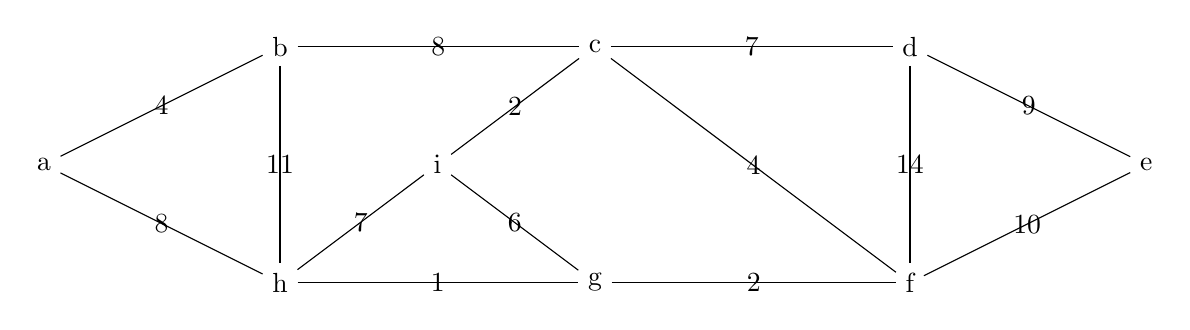
\begin{tikzpicture}
			\begin{scope}\globalnodeset
				\node (a) at (0,0) {a};

				\node (b) at (3,1.5) {b};
				\node (h) at (3,-1.5) {h};

				\node (i) at (5,0) {i};

				\node (c) at (7,1.5) {c};
				\node (g) at (7,-1.5) {g};

				\node (d) at (11,1.5) {d};
				\node (f) at (11,-1.5) {f};

				\node (e) at (14,0) {e};
			\end{scope}
			\begin{scope}\globalpathset
				\path (a) edge node {$4$} (b);
				\path (a) edge node {$8$} (h);

				\path (b) edge node {$11$} (h);
				\path (b) edge node {$8$} (c);

				\path (h) edge node {$7$} (i);
				\path (h) edge node {$1$} (g);

				\path (i) edge node {$2$} (c);
				\path (i) edge node {$6$} (g);

				\path (c) edge node {$7$} (d);
				\path (c) edge node {$4$} (f);

				\path (g) edge node {$2$} (f);

				\path (d) edge node {$14$} (f);
				\path (d) edge node {$9$} (e);

				\path (f) edge node {$10$} (e);
			\end{scope}
		\end{tikzpicture}
		\label{fig:26.2}
	\end{figure}
	\begin{answer}
		\begin{table}
			\centering
			\begin{threeparttable}
				\label{tab:mst-example}
				\begin{tabular}{c|c}
					\textbf{Node} & \textbf{Visited?}\\
					\midrule
					$a$ & \\
					$b$ & \\
					$c$ & Visited\\
					$d$ & \\
					$e$ & \\
					$f$ & \\
					$g$ & \\
					$h$ & \\
					$i$ & \\
				\end{tabular}
				\begin{tablenotes}
					\small
					\item Started at $c$.
				\end{tablenotes}
			\end{threeparttable}
	\end{table}
	\end{answer}
\end{enumerate}

\begin{answer}
	\begin{minipage}{0.5\textwidth}
		\begin{algorithm}[H]
			\caption{Prim's Algorithm (MST)}\label{alg:mst-prim}
			\begin{algorithmic}[1]
				\Function{MST-Prim}{$G$, W, $r$}
					\ForAll{$u\in G.V$}
						\State $u.key\gets\infty$
						\State $u.\pi \gets $ NIL
					\EndFor
					\State $r.key\gets0$
					\State $Q\gets G.B$
					\While{$Q\neq\emptyset$}
						\State $u\gets\Call{\hyperref[subsec:Extract-Min]{Extract-Min}}{Q}$
						\ForAll{$v\in G.Adj[u]$}
							\If{$v\in Q$ and $\Call{w}{u,v} < v.key$}
								\State $v.\pi\gets u$
								\State $v.key\gets \Call{w}{u,v}$
							\EndIf
						\EndFor
					\EndWhile
				\EndFunction
			\end{algorithmic}
		\end{algorithm}
	\end{minipage}%
	\begin{minipage}{0.5\textwidth}
		\begin{algorithm}[H]
			\caption{Kruskal's Algorithm (MST)}\label{alg:mst-kruskal}
			\begin{algorithmic}[1]
				\Function{MST-Kruskal}{$G$, $w$}
					\State $A\gets\emptyset$
					\ForAll{vertex $v\in V[G]$}
						\State \Call{Make-Set}{$v$}
					\EndFor
					\State sort the edges of $E$ into increasing
					\ForAll{edge $(u,v)\in E$, taken in increasing order}
						\If{$\Call{Find-Set}{u}\neq\Call{Find-Set}{v}$}
							\State $A\gets A\cup \left\{ (u,v) \right\}$
							\State \Call{Union}{$u$,$v$}
						\EndIf
					\EndFor
				\EndFunction
			\end{algorithmic}
		\end{algorithm}
		~\\
	\end{minipage}
\end{answer}

Demonstration of Prim (Deleted): \url{http://en.wikipedia.org/wiki/File:Prim-algorithm-animation-2.gif}

Demonstration of Kruskal: \url{https://www.cs.usfca.edu/~galles/visualization/Kruskal.html}\\
\newcommand{\stepupcounter}[1]{\stepcounter{#1}\arabic{#1}}
\newcounter{kruskal}
\newcommand{\mstcaption}[3]{Connected vertices $#1$ and $#2$ with an edge with weight $#3$.}

\begin{answer}
	\begin{figure}[H]
		\centering
		\begin{tikzpicture}
			\begin{scope}\globalnodeset
				\node (a) at (0,0) {a};

				\node (b) at (3,1.5) {b};
				\node (h) at (3,-1.5) {h};

				\node (i) at (5,0) {i};

				\node (c) at (7,1.5) {c};
				\node (g) at (7,-1.5) {g};

				\node (d) at (11,1.5) {d};
				\node (f) at (11,-1.5) {f};

				\node (e) at (14,0) {e};
			\end{scope}
			\begin{scope}\pathset
				\path (a) edge node {$4$} (b);
				\path (a) edge node {$8$} (h);

				\path (b) edge node {$11$} (h);
				\path (b) edge node {$8$} (c);

				\path (h) edge node {$7$} (i);
				\path [thickedge] (h) edge node {$1$} (g);

				\path (i) edge node {$2$} (c);
				\path (i) edge node {$6$} (g);

				\path (c) edge node {$7$} (d);
				\path (c) edge node {$4$} (f);

				\path (g) edge node {$2$} (f);

				\path (d) edge node {$14$} (f);
				\path (d) edge node {$9$} (e);

				\path (f) edge node {$10$} (e);
			\end{scope}
		\end{tikzpicture}
		\caption{\mstcaption{h}{g}{1}}
		\label{fig:kruskal-example-a}
	\end{figure}
	\begin{figure}[H]
		\centering
		\begin{tikzpicture}
			\begin{scope}\globalnodeset
				\node (a) at (0,0) {a};

				\node (b) at (3,1.5) {b};
				\node (h) at (3,-1.5) {h};

				\node (i) at (5,0) {i};

				\node (c) at (7,1.5) {c};
				\node (g) at (7,-1.5) {g};

				\node (d) at (11,1.5) {d};
				\node (f) at (11,-1.5) {f};

				\node (e) at (14,0) {e};
			\end{scope}
			\begin{scope}\pathset
				\path (a) edge node {$4$} (b);
				\path (a) edge node {$8$} (h);

				\path (b) edge node {$11$} (h);
				\path (b) edge node {$8$} (c);

				\path (h) edge node {$7$} (i);
				\path [thickedge] (h) edge node {$1$} (g);

				\path [thickedge] (i) edge node {$2$} (c);
				\path (i) edge node {$6$} (g);

				\path (c) edge node {$7$} (d);
				\path (c) edge node {$4$} (f);

				\path (g) edge node {$2$} (f);

				\path (d) edge node {$14$} (f);
				\path (d) edge node {$9$} (e);

				\path (f) edge node {$10$} (e);
			\end{scope}
		\end{tikzpicture}
		\caption{\mstcaption{c}{i}{2}}
		\label{fig:kruskal-example-b}
	\end{figure}
	\begin{figure}[H]
		\centering
		\begin{tikzpicture}
			\begin{scope}\globalnodeset
				\node (a) at (0,0) {a};

				\node (b) at (3,1.5) {b};
				\node (h) at (3,-1.5) {h};

				\node (i) at (5,0) {i};

				\node (c) at (7,1.5) {c};
				\node (g) at (7,-1.5) {g};

				\node (d) at (11,1.5) {d};
				\node (f) at (11,-1.5) {f};

				\node (e) at (14,0) {e};
			\end{scope}
			\begin{scope}\pathset
				\path (a) edge node {$4$} (b);
				\path (a) edge node {$8$} (h);

				\path (b) edge node {$11$} (h);
				\path (b) edge node {$8$} (c);

				\path (h) edge node {$7$} (i);
				\path [thickedge] (h) edge node {$1$} (g);

				\path [thickedge] (i) edge node {$2$} (c);
				\path (i) edge node {$6$} (g);

				\path (c) edge node {$7$} (d);
				\path (c) edge node {$4$} (f);

				\path [thickedge] (g) edge node {$2$} (f);

				\path (d) edge node {$14$} (f);
				\path (d) edge node {$9$} (e);

				\path (f) edge node {$10$} (e);
			\end{scope}
		\end{tikzpicture}
		\caption{\mstcaption{g}{f}{2}}
		\label{fig:kruskal-example-c}
	\end{figure}
	\begin{figure}[H]
		\centering
		\begin{tikzpicture}
			\begin{scope}\globalnodeset
				\node (a) at (0,0) {a};

				\node (b) at (3,1.5) {b};
				\node (h) at (3,-1.5) {h};

				\node (i) at (5,0) {i};

				\node (c) at (7,1.5) {c};
				\node (g) at (7,-1.5) {g};

				\node (d) at (11,1.5) {d};
				\node (f) at (11,-1.5) {f};

				\node (e) at (14,0) {e};
			\end{scope}
			\begin{scope}\pathset
				\path [thickedge] (a) edge node {$4$} (b);
				\path (a) edge node {$8$} (h);

				\path (b) edge node {$11$} (h);
				\path (b) edge node {$8$} (c);

				\path (h) edge node {$7$} (i);
				\path [thickedge] (h) edge node {$1$} (g);

				\path [thickedge] (i) edge node {$2$} (c);
				\path (i) edge node {$6$} (g);

				\path (c) edge node {$7$} (d);
				\path (c) edge node {$4$} (f);

				\path [thickedge] (g) edge node {$2$} (f);

				\path (d) edge node {$14$} (f);
				\path (d) edge node {$9$} (e);

				\path (f) edge node {$10$} (e);
			\end{scope}
		\end{tikzpicture}
		\caption{\mstcaption{a}{b}{4}}
		\label{fig:kruskal-example-d}
	\end{figure}
	\begin{figure}[H]
		\centering
		\begin{tikzpicture}
			\begin{scope}\globalnodeset
				\node (a) at (0,0) {a};

				\node (b) at (3,1.5) {b};
				\node (h) at (3,-1.5) {h};

				\node (i) at (5,0) {i};

				\node (c) at (7,1.5) {c};
				\node (g) at (7,-1.5) {g};

				\node (d) at (11,1.5) {d};
				\node (f) at (11,-1.5) {f};

				\node (e) at (14,0) {e};
			\end{scope}
			\begin{scope}\pathset
				\path [thickedge] (a) edge node {$4$} (b);
				\path (a) edge node {$8$} (h);

				\path (b) edge node {$11$} (h);
				\path (b) edge node {$8$} (c);

				\path (h) edge node {$7$} (i);
				\path [thickedge] (h) edge node {$1$} (g);

				\path [thickedge] (i) edge node {$2$} (c);
				\path (i) edge node {$6$} (g);

				\path (c) edge node {$7$} (d);
				\path [thickedge] (c) edge node {$4$} (f);

				\path [thickedge] (g) edge node {$2$} (f);

				\path (d) edge node {$14$} (f);
				\path (d) edge node {$9$} (e);

				\path (f) edge node {$10$} (e);
			\end{scope}
		\end{tikzpicture}
		\caption{\mstcaption{c}{f}{4}}
		\label{fig:kruskal-example-e}
	\end{figure}
	\begin{figure}[H]
		\centering
		\begin{tikzpicture}
			\begin{scope}\globalnodeset
				\node (a) at (0,0) {a};

				\node (b) at (3,1.5) {b};
				\node (h) at (3,-1.5) {h};

				\node (i) at (5,0) {i};

				\node (c) at (7,1.5) {c};
				\node (g) at (7,-1.5) {g};

				\node (d) at (11,1.5) {d};
				\node (f) at (11,-1.5) {f};

				\node (e) at (14,0) {e};
			\end{scope}
			\begin{scope}\pathset
				\path [thickedge] (a) edge node {$4$} (b);
				\path (a) edge node {$8$} (h);

				\path (b) edge node {$11$} (h);
				\path (b) edge node {$8$} (c);

				\path (h) edge node {$7$} (i);
				\path [thickedge] (h) edge node {$1$} (g);

				\path [thickedge] (i) edge node {$2$} (c);
				\path (i) edge node {$6$} (g);

				\path [thickedge] (c) edge node {$7$} (d);
				\path [thickedge] (c) edge node {$4$} (f);

				\path [thickedge] (g) edge node {$2$} (f);

				\path (d) edge node {$14$} (f);
				\path (d) edge node {$9$} (e);

				\path (f) edge node {$10$} (e);
			\end{scope}
		\end{tikzpicture}
		\caption{\mstcaption{c}{d}{7}}
		\label{fig:kruskal-example-f}
	\end{figure}
	\begin{figure}[H]
		\centering
		\begin{tikzpicture}
			\begin{scope}\globalnodeset
				\node (a) at (0,0) {a};

				\node (b) at (3,1.5) {b};
				\node (h) at (3,-1.5) {h};

				\node (i) at (5,0) {i};

				\node (c) at (7,1.5) {c};
				\node (g) at (7,-1.5) {g};

				\node (d) at (11,1.5) {d};
				\node (f) at (11,-1.5) {f};

				\node (e) at (14,0) {e};
			\end{scope}
			\begin{scope}\pathset
				\path [thickedge] (a) edge node {$4$} (b);
				\path [thickedge] (a) edge node {$8$} (h);

				\path (b) edge node {$11$} (h);
				\path (b) edge node {$8$} (c);

				\path (h) edge node {$7$} (i);
				\path [thickedge] (h) edge node {$1$} (g);

				\path [thickedge] (i) edge node {$2$} (c);
				\path (i) edge node {$6$} (g);

				\path [thickedge] (c) edge node {$7$} (d);
				\path [thickedge] (c) edge node {$4$} (f);

				\path [thickedge] (g) edge node {$2$} (f);

				\path (d) edge node {$14$} (f);
				\path (d) edge node {$9$} (e);

				\path (f) edge node {$10$} (e);
			\end{scope}
		\end{tikzpicture}
		\caption{\mstcaption{a}{h}{8}}
		\label{fig:kruskal-example-g}
	\end{figure}
	\begin{figure}[H]
		\centering
		\begin{tikzpicture}
			\begin{scope}\globalnodeset
				\node (a) at (0,0) {a};

				\node (b) at (3,1.5) {b};
				\node (h) at (3,-1.5) {h};

				\node (i) at (5,0) {i};

				\node (c) at (7,1.5) {c};
				\node (g) at (7,-1.5) {g};

				\node (d) at (11,1.5) {d};
				\node (f) at (11,-1.5) {f};

				\node (e) at (14,0) {e};
			\end{scope}
			\begin{scope}\pathset
				\path [thickedge] (a) edge node {$4$} (b);
				\path [thickedge] (a) edge node {$8$} (h);

				\path (b) edge node {$11$} (h);
				\path (b) edge node {$8$} (c);

				\path (h) edge node {$7$} (i);
				\path [thickedge] (h) edge node {$1$} (g);

				\path [thickedge] (i) edge node {$2$} (c);
				\path (i) edge node {$6$} (g);

				\path [thickedge] (c) edge node {$7$} (d);
				\path [thickedge] (c) edge node {$4$} (f);

				\path [thickedge] (g) edge node {$2$} (f);

				\path (d) edge node {$14$} (f);
				\path [thickedge] (d) edge node {$9$} (e);

				\path (f) edge node {$10$} (e);
			\end{scope}
		\end{tikzpicture}
		\caption{\mstcaption{d}{e}{9}}
		\label{fig:kruskal-example-h}
	\end{figure}
\end{answer}
%</Lecture-Activity-26>

\end{document}